\documentclass[10pt]{jarticle}
\usepackage[dvipdfmx]{graphicx}
\usepackage{amsmath}
\usepackage{comment}
\usepackage{setspace}
\usepackage{float}
\usepackage{indentfirst}
\usepackage{here}
\usepackage{caption}
\usepackage{multicol}

\captionsetup[figure]{font=footnotesize}

\setlength{\hoffset}{0cm}
\setlength{\oddsidemargin}{-15mm}
\setlength{\evensidemargin}{-3cm}
\setlength{\marginparsep}{0cm}
\setlength{\marginparwidth}{0cm}
\setlength{\textheight}{26.7cm}
\setlength{\textwidth}{19cm}
\setlength{\topmargin}{-50pt}      % 上の余白を調整
\setlength\abovecaptionskip{0pt}

\renewcommand{\baselinestretch}{1.0}
\renewcommand{\floatpagefraction}{1}
\renewcommand{\topfraction}{1}
\renewcommand{\bottomfraction}{1}
\renewcommand{\textfraction}{0}
\renewcommand{\labelenumi}{(\arabic{enumi})}
\renewcommand{\figurename}{Fig.} %図をFig.にする(画像のとこだけ)

\begin{comment}
  %図のキャプションからコロン:を消す
  \makeatletter
  \long\def\@makecaption#1#2{% #1=図表番号,#2=キャプション本文
    \sbox\@tempboxa{#1. #2}
    \ifdim \wd\@tempboxa >\hsize
    #1 #2\par 
    \else
    \hb@xt@\hsize{\hfil\box\@tempboxa\hfil}
    \fi
  }  
  \makeatother 
\end{comment}

%%sectionの前後の余白を消す
\makeatletter
\def\section{\@startsection {section}{1}{\z@}{-0.5ex plus -1ex minus -.2ex}{0.5 ex plus .2ex}{\small\bf}}
\def\subsection{\@startsection {subsection}{1}{\z@}{-0.5ex plus -1ex minus -.2ex}{0.5 ex plus .2ex}{\small\bf}}
\def\subsubsection{\@startsection {subsubsection}{1}{\z@}{-0.5ex plus -1ex minus -.2ex}{0.5 ex plus .2ex}{\footnotesize\bf}}
\makeatother

\pagestyle{myheadings}
%\pagestyle{empty} % すべてのページ番号を消去

\begin{document}
%文字サイズ
%\scriptsize   %7pt
\footnotesize %8pt
%\small        %9pt

\markright{第 16 回全日本学生フォーミュラ大会 Car No.029 九州工業大学デザインレポート}
%%\multicolumn{1}{|c|}{\includegraphics[width=10mm]{figure/eps/Logo.eps}}

%% \markleft{
%%   \includegraphics[width=10mm]{figure/eps/Logo.eps}
%% }

\date{\vspace{-15mm}}
\title{\vspace{-18mm} \small Car No.029 Kyushu Institute of Technology KIT-formula Design Report}

\oddsidemargin = -15mm
\maketitle % 実際の表題の出力
\thispagestyle{empty}
%\tableofcontents

%タイトル
%% \begin{center}
%%   {ji}
%% \end{center}


%\newpage
%イントロ
昨年度のKIT-formulaでは,2017年度大会において総合32位という結果に終わり,目標としていた歴代最高順位の8位を超える6位入賞を達成することが出来なかった.
したがって今年度では,根本的な車両の成り立ちを見直し,昨年度車両(以下KS-14)よりも確実に速く,勝てる車両を目指した.
そこで今年度の車両コンセプトを,昨年度よりも数段速い車両を意味し,また新たなことに挑戦するというチームの想いを込めた「Speed Evolution」とし,シングルナンバー(総合順位一桁)を目標に今年度車両(以下KS-15)の開発を行った.


\begin{multicols}{2}
%コンセプト
%%%%%%%%%%%%%%%%%%%%%%%%%%%
\section{車両開発方針}
%%%%%%%%%%%%%%%%%%%%%%%%%%%
車両開発の目標であるシングルナンバーを獲得するため,動的競技のうち最も総合順位との相関のあるエンデュランスに着目した.過去3年の大会結果から,総合順位一桁のチームはエンデュランスにおいても高順位であることが分かった.そこで昨年度の結果から,エンデュランス総合タイムが1320 sec(平均タイム66.0 sec/lap)で総合順位が8位以上を獲得できることが分かったため,これを車両開発目標に設定し開発を行った.

%%%%%%%%%%%%%%%%%%%%%%%%%%%
\subsection{ベンチマーク分析}
%%%%%%%%%%%%%%%%%%%%%%%%%%%
前項にて設定したエンデュランス総合タイムで走行していた2017年度大会の他大学車両と,KS-14との間でどういった区間でタイム差が生じているかをベンチマークとして,昨年度大会の動画から検証を行った.動画から区間A,Bを設定し(区間A:高速状態での加速性能,旋回性能が重視される区間,区間B:低速からの加速性能,応答性能が重視される区間)分析を行ったところ,区間Aでは平均して$\Delta$1.557 sec,区間Bでは$\Delta$2.379 secと,KS-14とベンチマークとの間に差があることが分かった.そこでパワートレインでは主にエンジン低回転領域からの加速性能,サスペンションでは旋回性能に加え応答性能を重視して開発を行った.またフレームやエアロデバイスといったボディではサスペンションの性能要求を満たすこと,コクピットにおいては従来のDrivabilityに加え,今まで重要視していなかったドライバーの快適性(以下Comfortability)を追求することとした.またサスペンションからの性能要求を満たすため,各パーツにおいて軽量化の検討を行った.


%サスペンション
%%%%%%%%%%%%%%%%%%%%%%%%%%%
\section{サスペンション}
%%%%%%%%%%%%%%%%%%%%%%%%%%%
チーム目標であるシングルナンバーを獲得するためにサスペンション系では前述のコース,タイム分析からコーナーの定常領域で0.54 sec,過渡領域であるパイロンスラロームにおいて1.84 secの短縮が必要であることが分かった.

%suspension
%%%%%%%%%%%%%%%%%%%%%%%%%%%
\subsection{subtitle}
%%%%%%%%%%%%%%%%%%%%%%%%%%%
あいうえお(Fig.\ref{fig:label1}).

かきくけこ(Fig.\ref{fig:label2}).



%hubs
%% %%%%%%%%%%%%%%%%%%%%%%%%%%%
%% \subsection{ハブ}
%% %%%%%%%%%%%%%%%%%%%%%%%%%%%
%% KS-15では軽量化することで慣性モーメントを減少させるためハブベアリングの重量を削減した.KS-15のハブベアリングはKS-14と比較すると外径が-10 mm,重量が-125 gとなり小型化を実現した.また,Rr.ハブの形状を見直し,剛性を保ちつつ-7 gの軽量化を行った.


%uplights
\input{subfiles/suspension/uplights/uplights.tex}


%ボディ
%%%%%%%%%%%%%%%%%%%%%%%%%%%
\section{ボディ}
%%%%%%%%%%%%%%%%%%%%%%%%%%%
aaaaaaaaaaaaaaaaaaaaaaaa

%ボディ
%%%%%%%%%%%%%%%%%%%%%%%%%%%
\section{フレーム}
%%%%%%%%%%%%%%%%%%%%%%%%%%%
フレームでは,全体目標であるエンデュランス1320 secの達成の為に車両応答性の向上に加え,コクピット班の目標であるComfortabilityの向上を目標として設計を行った.

まず設計を行う前に,フレームが車両挙動に及ぼす影響を調べるためにKS-14のねじり剛性,横曲げ剛性を変化させて舵角,横G,右側後輪のダンパーのストローク量を模擬コースの走行により測定を行った.この結果,最も横Gが大きかったスラローム区間においてデータを比較したところ,Fig.\ref{fig:frame1}に示すように右側の後輪に取り付けたストロークセンサーから横Gに対する変位量は剛性に対してほぼ変化が無いという結果が得られた.次に操舵に対する横Gの位相を調べたところ,剛性が増加するにつれて位相の遅れが小さくなっていることが確認できた.この応答性は横曲げ剛性に起因すると考え,’18年度はフレームの横曲げ剛性を向上させることにより,操舵に対する横Gの位相遅れを小さくすることを目標にした.

%%%%%%%%%%%%%%%%%%%%%%%%%%%
\subsection{設計概要}
%%%%%%%%%%%%%%%%%%%%%%%%%%%
上述の目標から,KS-15ではKS-14からフレームの重量を変化させず,その中で可能な限り横曲げ剛性を向上させるように設計を行った.その結果’18年度の重量と横曲げ剛性はCATIA上でそれぞれ31.2 kg,16×10$^5$ N-mとなり,前年度の31.1 kg,9×10$^5$ N-mから重量をほぼ変化させずに横曲げ剛性を7×10$^5$ N-m向上させることが出来た.また,設計通りの性能を発揮させるためには,旋回時のサスペンションの動きを設計に忠実に動作させる必要があると考えた.そこで,Aアームやトーロッドのフレーム取り付け部の変位を抑えるため,前年度と同様に取り付け部を可能な限りフレームのノードに取り付けられるように設計を行うことに加え,取り付けられなかった箇所については小径パイプにより変位を抑えた.

次にComfortabilityの向上について,シートと共同で設計を進めドライバーの姿勢を決定した後にフレームのレイアウトの設計を行った.これにより,全年度フレームに比べてシートステイロア部分の幅を330 mmから430 mmに増加させシートの幅を十分に取れるように変更した.また,Fr.フープの上部に新たに曲げを入れることによりステアリングの位置を上げつつドライバーの視界を確保することができた.


%エアロ
%%%%%%%%%%%%%%%%%%%%%%%%%%%
\section{エアロ}
%%%%%%%%%%%%%%%%%%%%%%%%%%%
\label{sec:concept}
%%問題点
KS-14はサイドポンツーンを搭載しなかった.その影響でラジエータは必要な空気の流入量を確保できず,昨年の大会では水温が$110 \ {}^\circ\mathrm{C}$にまで上昇した.また,KS-14はアンダーステアの傾向にあり,コーナー脱出直後にアクセルを踏み込むことができなかった.

%% %%改善点
%% KS-15はこれらの問題を解決するべく,KS-14の空力デバイスに加え,「サイドポンツーン」「ウイング」を新たに搭載する.これは,サイドポンツーンによる導風によってラジエータに流れ込む空気を確保し,Fr.ウイングによるDF(以下 DF)によってFr.タイヤのCFを増大させることが狙いである.また,Fr.ウイングのみを搭載すると,マシンの姿勢変化によるDFの変動によってマシンの荷重移動が顕著になり,Drivabilityの低下につながると考え,Rr.ウイングも搭載することによって前後のウイングによる空力重心を適切な位置に置き,荷重移動の抑制とDrivabilityの向上を狙う.さらに,サスペンション班からの要求として,空力デバイスによる総DF:150Nと,目標重量4.5N/kgを満たすウイングを目標とする.

%%改善点(坂井さん案)
KS-15はこれらの問題を解決するべく,KS-14の空力デバイスに加え,「サイドポンツーン」「ウイング」を新たに搭載する.これは,サイドポンツーンによる導風によってラジエータに流れ込む空気を確保し,Fr.ウイングによるDFによってFr.タイヤのCFを増大させることが狙いである.

また,車体バネ上重心とピッチ中心位置関係による車体バネ上重量の荷重移動と,姿勢変化(制動Frダイブ\&加速ピッチング)による空力重心の移動をうまくバランスさせることで,マシンのコーナリング性能の上昇を狙うためにRr.ウイングも搭載することにした.

さらに,サスペンションからの要求より,空力デバイスによる総DF:150 Nと,重量4.5 N/kgを満たすウイングを目標とする.

%%解析に関して
解析はソフトウェアクレイドル社の三次元熱流体解析ソフトSCRYU/Tetraを使用した.解析条件はアクセラレーションとスキッドパッドの状況を想定して行った.より正確な解析結果を得るために,速度は走行時の平均速度である40 km/hを基本とし,解析モデルにはヘルメットやヘッドレスト周辺のファイアウォールなどを組み込んだ.また,走行状態を再現するためにタイヤと路面には速度に応じた回転や移動条件を与え,スキッドパッドでは舵角とスリップアングルも再現した.

%%%%%%%%%%%%%%%%%%%%%%%%%%%
\subsection{Fr.ノーズ}
%%%%%%%%%%%%%%%%%%%%%%%%%%%
%% \subsection{問題と改善点}
%% %%%%%%%%%%%%%%%%%%%%%%%%%%%
%% KS-14のCFD解析結果より,ノーズ先端に高い圧力が広範囲にかかっていることがわかった.よって,高い圧力がかかる範囲を少なくするために,KS-15ではKS-14よりも先端を鋭利なものにした.CFD解析による,KS-14とKS-15のノーズにかかる表面圧力の比較をFig.○に示す.

%%%%%%%%%%%%%%%%%%%%%%%%%%%
\subsubsection{製作方法の改善}
%%%%%%%%%%%%%%%%%%%%%%%%%%%
KS-14のFr.ノーズは歪んでおり,設計通りに製作できたとは言えなかった.KS-14は断面図を貼り付けたネオマフォームに合わせて型を成型していたため,型を成型する際に目標とする形状を視認することができず,型に歪みが生じたと考えた.そこでKS-15では成型を行う前に木材の板を用いてFr.ノーズの目標とする形状を再現した.木材の切り出しはレーザーカッターを用いることで製作精度が向上した.成型を行う前に形状を再現することによって,目標とする形状を確認しながら成型することができた.この製作方法によってFr.ノーズの歪みを改善することができ,KS-14ではすべて人の手で行っていた作業を,KS-15では一部の工程にレーザーカッターを用いることで型の修正にかかる時間を短縮することができたため,製作期間を40 \%短縮することができた.

%%%%%%%%%%%%%%%%%%%%%%%%%%%
\subsection{サイドポンツーン\&サイドパネル}
%%%%%%%%%%%%%%%%%%%%%%%%%%%
CFD解析によるサイドポンツーン周辺の空気の流れをFig.\ref{fig:pontoon}に示す.

まず,KS-14の冷却性能の課題を改善するため,KS-15ではサイドポンツーンとサイドパネルを搭載した.サイドポンツーンはFr.タイヤ後方に位置するため,形状によっては回転によって生じるタイヤ後方の乱流がサイドポンツーンに流れ込み,ラジエータへの流量低下につながると考えた.したがって,サイドポンツーンの形状を,ノーズとFr.タイヤの間から来る空気を積極的に取り込むような形状とした.

また,KS-14ではコクピット内への空気の流入を防ぐために,側面下部にのみパネルを貼っていた.しかし,塞がれていない側面上部からコクピット内へ空気が流入し,空気の流れを妨げていることがCFD解析によりわかった.そこでKS-15ではこの流入を防ぐために,側面をサイドパネルで覆った.

%% %%%%%%%%%%%%%%%%%%%%%%%%%%%
%% \subsection{サイドパネル}
%% %%%%%%%%%%%%%%%%%%%%%%%%%%%
%% KS-14ではコックピット内への空気の流入を防ぐために,側面下部にのみパネルを貼っていた.しかし,塞がれていない側面上部からコックピット内へ空気が流入し,空気の流れを妨げていることがCFD解析によりわかった.そこでKS-15ではこの流入を防ぐために,側面をサイドパネルで覆った.

%%%%%%%%%%%%%%%%%%%%%%%%%%%
\subsection{ウイング}
%%%%%%%%%%%%%%%%%%%%%%%%%%%
\subsubsection{翼断面形状の決定}
%%%%%%%%%%%%%%%%%%%%%%%%%%%
%%迎角変化
KS-15の翼型はNACA-97をベースにCFD解析を行いながら設計した.NACAのレポート\cite{NACA}によると,NACA-97は迎角15$^\circ$のときにCl値が,迎角-2$^\circ$のときにCd値がそれぞれピークに達する.KS-14の平均速度40 km/hにおいて,NACA-97の迎角の変化に対する各パラメータの変化をCFD解析によって調べるとFig.\ref{fig:angle_data}のようになった.ウイングによるDFはコーナー進入時に最も必要であると考え,ブレーキング終点の姿勢変化において,KS-15で使用するウイングのメインフラップの迎角がFig.\ref{fig:angle_data}のCl値が急に落ち込む15$^\circ$となるようにした.

%%スリット
次に,NACA-97の迎角20$^\circ$のときの乱流エネルギーの分布をFig.\ref{fig:naca97_deg20}に示す.このときCl値は3.50,Cd値は0.76,L/Dは4.61であった.ウイングは迎角やキャンバーを大きくしていくことで,ウイング裏面の反り返りが強くなり,空気の剥離が起こる.空気の剥離が起こることによってウイング後方には負圧が発生し,それにより生じる圧力抗力が空気抵抗となる.迎角20$^\circ$のときのNACA-97にも同様の現象が見られたため,空気の剥離点付近にスリットを設けることでウイング前方から後方へ空気を送りこみ,空気の剥離を抑えた.迎角20$^\circ$の一枚翼にスリットを設けて三分割した翼断面の乱流エネルギーの分布をFig.\ref{fig:naca97_151515}に示す.CFD解析の結果より,スリットを設けることで空気の剥離は改善され,一枚翼と比べてCl値は5.26となり50 \%,Cd値は1.03となり0.36 \%上昇した.L/Dは5.11となり,0.11 \%上昇した.

以上の解析で得られたデータを用いてウイングの翼断面の形状を決定した.

%%%%%%%%%%%%%%%%%%%%%%%%%%%
\subsubsection{Fr.ウイング}
%%%%%%%%%%%%%%%%%%%%%%%%%%%
%%立ち位置的な
Fr.ウイングは%マシンの中で最初に風に接触する部分であり,Fr.ウイングから%
後方のパーツの空気の流れに影響を与える重要なパーツである.また,地面に最も近い位置に存在するため,グランドエフェクトによるDF増加も期待できると考える.

%%形状
KS-15のFr.ウイングの概形はサイドポンツーンに流入する風の向きを妨げないように,ノーズ付近のフラップを低くした.

翼端板はタイヤ後方に生じる乱流を減らす目的で外側へ反らす形状とすることで空気がタイヤに衝突しづらくし,かつフラップ下方の空気の流速を速めることを狙った,さらにフラップ下方の負圧に向かって外から空気が流れこむのを防ぐためにフットフランジを設けた.

翼端板と同様の目的で,コーナリング時に空気がタイヤに衝突しづらくなるように,フラップ下方にスプリッターを設けた.

%%また,タイヤ直前に位置するフラップによってはね上げられた空気はタイヤ上方に衝突する.この衝突によって,タイヤ後方に乱流が生じ

%% 風の向きとタイヤ表面の進行方向が逆であるため,摩擦抗力が生じ,摩擦によってタイヤ温度の過度な上昇につながることが考えられる.そこで,フラップの両端に壁を設けて空気の流れを制限するのではなく,フラップ上面を流れる空気を横へ逃がし,タイヤに衝突する空気の量を減らす目的でフラップの両端のうち,内側の壁を除いた.CFD解析による,壁を設けた場合と除いた場合のタイヤの表面圧力の比較をFig.\ref{fig:tire_acc}とFig.\ref{fig:tire_skid}に示す.

%% タイヤ正面の正圧によって空気の剥離が起きやすくなると考え,空気の剥離を抑えるために,Fr.ウイングの翼端板の形状をウイングの外から空気を送り込むようにした.%%よく分かってないけどね

%%最低地上高
Fr.ウイングの最低地上高はグランドエフェクトによるDFを得るために,ボディの最低地上高よりも5 mmの余裕を持って35 mmとした.

%%%%%%%%%%%%%%%%%%%%%%%%%%%
\subsubsection{Rr.ウイング}
%%%%%%%%%%%%%%%%%%%%%%%%%%%
%%立ち位置的な
Rr.ウイング前方にはメインフープ周辺のファイアウォールや吸気系パーツなど,空気の流れを妨げるものが多く存在するため,Rr.ウイングはそれらによって生じる乱流や負圧の影響を受けやすい.また,Rr.ウイングはFr.ウイングに比べて大規模なものにできるため,大きなDFを得やすい反面,前方投影面積の増大によるドラッグの増加も起こりやすいと考えられる.

%%マウント方法
バネ上マウントはマシンの姿勢変化によってRr.ウイングの迎角が変化すると考えた.したがってKS-15ではマシンの姿勢変化に影響を受けず,またサスペンションを経由することなく,直接タイヤにDFを印加できるバネ下マウントを採用した.

%%高さ
Rr.ウイング前方のパーツによって生じる乱流や負圧の影響を回避するために,Rr.ウイングは前方のパーツから離れた位置に配置したい.しかし,慣性モーメントは距離の二乗に比例するため,重心から離れた位置に配置すると,慣性モーメントの増加によってコーナリング性能に影響が及ぶ.KS-15のRr.ウイングはメインフープよりも低く設定し,バネ下マウントであることを考慮した上で可能な限り後方へ配置した.

%%%%%%%%%%%%%%%%%%%%%%%%%%%
\subsubsection{空力重心}
%%%%%%%%%%%%%%%%%%%%%%%%%%%
前後ウイングによって生じるモーメントがつり合う点を空力重心とし,この点がサスペンション班が定める前後重量比に近づくようにウイングを配置した.導出にはCFD解析によって得た前後ウイングそれぞれにかかるDFと空気による圧力モーメントを用いた.レギュレーションの範囲内でウイングの位置を調整し,空力重心を50:50とした.

%%%%%%%%%%%%%%%%%%%%%%%%%%%
\subsection{製作・解析精度の検証}
%%%%%%%%%%%%%%%%%%%%%%%%%%%
\label{sec:experiment}
製作精度の影響により,CFD解析と同じような結果が得られないことも考えられるため,製作・解析精度の検証を行った.検証はタフト法による流れの可視化を行った.

%と,センサによるDFと解析によるDFの比較を行った.

%%間に合えば書く.無理ならデザインパネルで話す
タフト法はRr.ウイングのフラップ下面に対して行った.検証結果をFig.\ref{fig:taft_acc},Fig.\ref{fig:taft_skid}に示す.

%ストロークセンサをFr.サスペンションに,歪みゲージをRr.ウイングのステーにそれぞれ取り付けて計測した.検証結果をFig.◯に示す.

%%%%%%%%%%%%%%%%%%%%%%%%%%%
\subsection{エアロ開発まとめ}
%%%%%%%%%%%%%%%%%%%%%%%%%%%
KS-14での問題点を改善するために,KS-15では新たな空力デバイスを追加した.デバイス単体でのCFD解析(@40 km/h)を行ったところ,Fr.ウイングはDF:62 N,L/D:4.7となり,Rr.ウイングはDF:95 N,L/D:3.8となることがわかった.しかし,空力デバイスをボディに搭載したモデルで解析をかけたところ,メインフープ後方にあるRr.ウイングがDF:85 N,L/D:2.9となり,単体での解析結果と比べてDFが11 \%減,L/Dが26 \%減となった.

\ref{sec:experiment}項で行ったタフト法の検証結果より,KS-15に搭載したRr.ウイングがメインフープ周辺パーツの影響を受け,本来の性能を引き出せていないのは明白である.ここで,ウイング単体での解析結果をサスペンションからの要求性能4.5 N/kgを適用すると,ウイングの目標重量はFr.ウイングは13 kg,Rr.ウイングは21 kgとなる.実際に制作したウイングはFr.ウイングは5 kg,Rr.ウイングは6.5 kgであるため,これらは\ref{sec:concept}項で述べたサスペンションの要求を達成している.

以上より,今後はマシン全体の流れに注目し,空力デバイスの性能を引き出すために「流れの一貫性」を確立することが課題になると考える.



%パワートレイン
%%%%%%%%%%%%%%%%%%%%%%%%%%%
\section{パワートレイン}
%%%%%%%%%%%%%%%%%%%%%%%%%%%
チーム目標を達成するためパワートレインのベンチマークよりも劣っている点を’17年度大会のエンデュランス区間タイムから分析を行った.
1.1項の分析の結果,低回転域からの加速性能がベンチマークよりも劣っていることが分かった.そこでパワートレインでは,更にその区間での分析を行い,1コーナーからストレートエンド到達までのタイム差がベンチマークよりも平均して0.4 sec遅く,最もタイムに影響を及ぼしていることに着目した.

ベンチマークでは上述の区間を60 mとすると,50 mを2.5 secで通過していることが分かった.従ってKS-15でのパワートレイン開発目標を,1コーナー脱出速度をロガーデータ等から40 km/hとし,「メインストレート50 mを2.5 secで走行可能な加速性能」とし開発を行った. 
またベンチマークの調査結果から,最高出力は最低80 PSを維持し,コーナー脱出時(低回転域)からの常用回転域でのトルク特性を重視した.常用回転域はKS-14のロガーデータ及びオンボード映像から5000~13000 rpmとした.

具体的には,まず吸気がKS-14の解析モデルをもとに設計を行い,それが終了次第排気が設計を行うという手順で行った.そして実走行において燃調セッティングにより解析値に近づける手法をとった.

%エンジン
%%%%%%%%%%%%%%%%%%%%%%%%%%%
\subsection{エンジン}
%%%%%%%%%%%%%%%%%%%%%%%%%%%
エンジンは,パワートレインの開発目標からメインストレートでの加速性能や最高速を重視した.したがって使用するエンジンは単気筒よりも出力の大きい4気筒エンジンとした.また昨年度との性能比較が容易といった観点から,KS-14と同様Kawasaki ZX-600PEとした。

%%%%%%%%%%%%%%%%%%%%%%%%%%%
\subsection{バルブタイミング}
%%%%%%%%%%%%%%%%%%%%%%%%%%%
パワートレインの開発目標を達成するため,常用回転域における最大トルク及び最高出力の向上を目標にバルブタイミングの再検討を行った.

KS-14では低回転域でのエンジン応答性向上やアイドリング安定による騒音の低減,再始動性向上を目的とし吸気側バルブタイミングを標準より22.5$^\circ$遅角させていた.しかし低回転域でのトルクや最高出力がダイナパック測定結果より悪化することが分かっていた.したがって,2017年度大会後にKS-14のエンジンモデルをGT-Power上で作成し標準バルブタイミングとの比較を行った.また出力と上述した目的の両立を狙い吸気側を14.4$^\circ$遅角及び排気側を14.4$^\circ$進角したものの検討も行った.Fig.\ref{fig:power1}がその結果である.これより22.5$^\circ$遅角すると最高出力発生点付近(14000 rpm)ではそこまで出力に差はないが,常用回転域全域でみると大幅に悪化することが分かった.次に吸気側を14.4$^\circ$遅角及び排気側を14.4$^\circ$進角したものについてもそこまでトルクの落ち込みを抑えることが出来なかった.ドライバーからのフィードバックやアクセラレーションの結果比較より,実走行においても応答性やタイムに望ましい結果が得られなかった.

アイドリングの安定や再始動性向上についてはMoTeCの本格導入やサイレンサの設計変更により対応可能であることから,今年度は常用回転域での出力を重視しバルブタイミングを標準とすることとした.


%吸気
%%%%%%%%%%%%%%%%%%%%%%%%%%%
\subsection{吸気}
%%%%%%%%%%%%%%%%%%%%%%%%%%%
昨年度の吸気系はサージタンク容量の増加とそれに伴う利用可能スペースの減少により,応答性の悪化と出力特性の低下を招いた.そこで,今年度の吸気の目標を応答性の向上と常用回転域における出力特性,特にコーナー脱出時(5000〜8000 rpm)における特性の向上とした.

%%%%%%%%%%%%%%%%%%%%%%%%%%%
\subsubsection{スロットルボディ}
%%%%%%%%%%%%%%%%%%%%%%%%%%%
スロットル径の検討について昨年までの径$\phi$25と一昨年の径$\phi$32のリストリクターを含めたモデルを三次元熱流体解析ソフトSCRYU/Tetraで定常解析を行った.スロットル開度ごとの質量流量を算出した結果,$\phi$25ではスロットル開度の増加に伴い質量流量が比較的線形で変化しているが,$\phi$32では質量流量は全体的に増加したがスロットル開度が80を超えると質量流量が減少した(Fig.\ref{fig:intake1}).また,GT-powerを用いた解析では$\phi$25と$\phi$32で出力特性に差は見られなかった.そこで,今年度は$\phi$25と$\phi$32のスロットルを製作し実走行にて評価を行った.

%%%%%%%%%%%%%%%%%%%%%%%%%%%
\subsubsection{スロットル径}
%%%%%%%%%%%%%%%%%%%%%%%%%%%
今年はGT-powerの解析結果によってスロットルの径を実走行での結果を基に決定するため,$\phi$25と$\phi$32のスロットルを製作した.これらのスロットルの形状は,ANSYS CFXでの解析結果を基に決定した.質量流量の向上を目標に設計する事により質量流量を昨年より最大で3.8 \%向上させることに成功した.

%%%%%%%%%%%%%%%%%%%%%%%%%%%
\subsubsection{出力特性}
%%%%%%%%%%%%%%%%%%%%%%%%%%%
GT-powerを用いて吸排気系でのパワー・トルク特性の評価を行った.吸排気での設計は吸気系がマシンの出力特性に及ぼす影響が大きいので吸気系の設計を先に行った.GT-powerでの設計は昨年度モデルからバルブタイミングの変更と吸気系のパラメータを変更し,主に吸気管長とタンク容量の決定を行った.ここで,吸気管長はファンネルから吸気ポートまでの距離のことを言い昨年度の130 mmから管長を長くしていった.その結果,Fig.\ref{fig:intake2}のように管長が280 mm,タンク容量3.5 Lの時にピークトルクが7000 rpmとなり5000〜8000 rpmにかけての出力特性を向上することができた.今後は実測による評価を行う予定である.

%%%%%%%%%%%%%%%%%%%%%%%%%%%
\subsubsection{サージタンク}
%%%%%%%%%%%%%%%%%%%%%%%%%%%
サージタンクの容量はGT-powerの解析による結果から3.5 Lに決定し,形状は流体解析ソフトANSYS CFXを用いて各気筒への吸気流量にばらつきがないように形状を決定した.その結果,Fig.\ref{fig:intake3}のように各気筒への吸気流量のバラつき2.5 \%以下に抑えることができた.


%排気
%%%%%%%%%%%%%%%%%%%%%%%%%%%
\subsection{排気}
%%%%%%%%%%%%%%%%%%%%%%%%%%%
排気系設計ではパワートレインの目標を達成するため常用回転域での更なるトルク向上と扱いやすい出力特性を目指し開発を行った.目標として常用回転域での最大軸トルクを60 N-mとした(前年度45N-m).加えて,ドライバーが扱いやすいリニアなトルク特性となるようにエンジンモデルを選定した.

またKS-14が孕んでいた様々な問題についても解決策を模索した.

%%%%%%%%%%%%%%%%%%%%%%%%%%%
\subsubsection{排気管}
%%%%%%%%%%%%%%%%%%%%%%%%%%%
まずKS-14の問題点として解析方法の未確立及び前年度との比較不足が挙げられた.これは,9月の段階にはGT-powerでKS-14のエンジンモデルを製作して解析を行い、比較対象を明確化することで解決した.次にKS-15では排気管の軽量化にも取り組み,排気系パーツ一つ一つの重量を実測・管理を徹底した.またKS-14から採用したはめ込み式の排気管は取り付けがしづらかったため,はめ込み式は踏襲しつつ集合部のみを一体形状とし整備性の向上に努めた.集合部は左右対称形状とすることで排気管の取り回し設計や製作を行いやすくした.またA/Fセンサーマウントを各気筒に配置することで,気筒別に燃調マッピングが行える構造とした.(Fig.\ref{fig:power3})

次に軸トルク向上及び扱いやすい出力特性を達成するため,吸気側が先に製作した’17年度エンジンモデルを参考に,主に排気管長と管径を変更しながら10個ほどのモデルを作成した.これらの解析結果から,管径よりも管長,特に集合部よりも前の管長(プライマリ)が出力特性に大きく影響を及ぼすことが分かった.そこで集合部以下を燃料タンクやフレームとの干渉を考慮しつつ必要最小限の管長・管径とした.管径については解析結果から僅かな差であるが$\phi$38.1が最適であったため,それ以降の解析は管長のみを変更し管径は常に$\phi$38.1で行った.以上の方法で約40個のモデルを作成し,その中から目標最大トルクを達成しかつリニアなトルク特性となるものを選定した.その結果プライマリ管長は495 mmとなった.Fig.\ref{fig:power4}にKS-14の標準バルブタイミングのものとKS-15のそれぞれのトルク・PS性能曲線を示す.Fig.\ref{fig:power4}から分かるように常用回転域において大幅にトルクが向上したことが分かる.また最大トルクは7500 rpmにおいて60.1 N-mとなり目標数値を達成した.また最小限の管長・管径としたことにより排気管で200 gの軽量化を実現することが出来た.

%%%%%%%%%%%%%%%%%%%%%%%%%%%
\subsubsection{サイレンサ}
%%%%%%%%%%%%%%%%%%%%%%%%%%%
KS-14においては,アイドリング時の騒音低減を狙ってチャンバー(サブサイレンサ)を搭載していた.しかしチャンバー単体で1200 gもあることに加えスペースを必要とするためサイレンサを外側に配置しなければならず慣性モーメントの増加を招いていた.そこでKS-15ではまずチャンバー廃止によるエンジン出力への影響を検討した.Fig.\ref{fig:power5}がGT-powerで解析した結果であるが,出力への影響は殆どなかったため廃止をすることに決定した.しかし騒音については全域において音圧レベルが増加することが解析結果から分かったため,増加分をサイレンサエンド部を延長することにより消音することとした.

サイレンサエンド部の長さを10 mmずつ長さの違うモデルを複数個作成しGT-powerを用いて評価・選定を行った.その結果,サイレンサエンド部が550 mmのときアイドリング時2500 rpmのとき100.2 dBC,11000 rpmのとき108.7 dBCとなり必要な消音性能を得ることが出来た(Fig.\ref{fig:power6}).


%電装
%%%%%%%%%%%%%%%%%%%%%%%%%%%
\section{title}
%%%%%%%%%%%%%%%%%%%%%%%%%%%
aaaaaaaaaaaaaa

%%%%%%%%%%%%%%%%%%%%%%%%%%%
\subsection{subtitle}
%%%%%%%%%%%%%%%%%%%%%%%%%%%
bbbbbbbbbbbbbb

%%%%%%%%%%%%%%%%%%%%%%%%%%%
\subsubsection{subsubtitle}
%%%%%%%%%%%%%%%%%%%%%%%%%%%
cccccccccccccc


%冷却
%%%%%%%%%%%%%%%%%%%%%%%%%%%
\subsection{冷却}
%%%%%%%%%%%%%%%%%%%%%%%%%%%
Fig.\ref{fig:radiator1}にKS-14とKS-15のラジエータ配置を示す.KS-15の冷却システムは十分な冷却性能の確保を設計方針とした.昨年のエンデュランスでは水温が$110 \ {}^\circ\mathrm{C}$を超えておりこれはラジエータの配置によるものと考えられた.KS-14はラジエータの外側が後方に倒れるように搭載していたがコア部に空気がうまく流入せず空気側の熱伝達率が小さくなっていると考えられる.これに対しKS-15はコア部が正面を向くように配置しサイドポンツーンの兼ね合いで25$^\circ$前傾させた.これによって熱伝達率の向上と放熱量の向上が見込める.またラジエータを正面に向けたため従来のサイズでは車幅を超えるためサイズを縮小したところの軽量化となった.またステーの見直しにより0.43 kg軽量化できた.


%燃料
%%%%%%%%%%%%%%%%%%%%%%%%%%%
\subsection{燃料}
%%%%%%%%%%%%%%%%%%%%%%%%%%%
’18年度のチーム目標を達成するためにはエンデュランス完走が前提であり,またパワートレインの目標を達成するためには燃料系の総重量は6000gを切る必要があると考えた.そこで,燃料システムの目標を「安定した燃料供給と軽量化」とした.なお,この総重量は“’18 年度目標マシン重量“に“マシン全体に対する燃料系の重量割合“を掛けて求めたものである.

これを踏まえて,製作目標は「エンデュランス完走直後の燃料残量の状態でコーナーに侵入した際でもエア噛みが発生しないタンク」とし,解析ソフトANSYSから得られた解析結果からこれに見合うタンクの形状および容量を決定した.その際の解析条件を,“タンク内に0.7 Lの燃料残量がある状態で最大横G 1.8 G及び最大縦G 0.5 Gが発生する”とした.なお,エンデュランス完走直後の燃料残量0.7 Lは,タンクの容量5.0 L(’15年度大会のタンク容量が5 Lだったことからこれを指標とした)から燃料の使用量4.3 L(気温$20 \ {}^\circ\mathrm{C}$時の試走会で測定した燃費により決定)を引いたものである. 

上記の解析条件よりタンクの形状を決定したが,形状の工夫だけでは旋回時に発生する液体の偏りを抑えることが出来ず,一時的ではあるがエア噛みが発生する瞬間があった.そこで,液体の偏り及び挙動を抑えるために’18年度から構造体内にバッフルプレートを設けることにした(Fig.\ref{fig:fuel1}).その結果,燃料残量0.7 L時に旋回Gが発生した際の液体の挙動が小さくなり,エア噛みの発生を抑えることが出来た(Fig.\ref{fig:fuel2}).これにより,燃料タンクの容量を17年度の5.3 Lから5.0 Lへの変更が可能になり,ガソリンを含めたのタンクの重量を311 g減少することに成功した.また,’17年度のタンクに使用したネックパイプの素材がA5052の$\phi$45 mm,t5 mmであったため,’18年度は同素材の$\phi$41 mm,t2 mmのものに変更することで330 gの軽量化に成功した.さらに,タンクに使用するプレートに曲げ加工を施すことで,タンクの1面につきアルミ板を1枚ずつ切り出すよりも溶接長が647 mm短くなり,179 g(溶接長1 mmにつき0.277 g)の軽量化に成功した.

したがって,’17年度と比較すると全体で990 g(実測値)の軽量化に成功し,’18年度燃料系の総重量はガソリン満タン時で5500 gとなり目標重量を達成した.



%エルゴノミクス
%コックピット
\input{subfiles/ergonomics/cockpit/cockpit.tex}

%シフター
%%%%%%%%%%%%%%%%%%%%%%%%%%%
\subsection{シフター}
%%%%%%%%%%%%%%%%%%%%%%%%%%%
KS-14のシフターはボタンのスイッチを使っていたためドライバーがボタンを押した感覚に乏しいという問題があった.またボタンをステアリング表面に配置していたため,シフト操作をする際に親指がステアリングから離れDrivabilityの悪化に繋がっていた.これの解決のためマイクロスイッチを用いたパドルシフトを使用しDrivabilityの改善を図った.シフトのアクチュエータに関しては引き続きKilictronicの電動シフターを使用し点火カットと併用することでシフトアップをクラッチを使用せず1モーションで行えるようにした。


%ペダル
%%%%%%%%%%%%%%%%%%%%%%%%%%%
\subsection{ペダルユニット}
%%%%%%%%%%%%%%%%%%%%%%%%%%%
%%問題点
昨年度は各ペダル共に足の指先部分での操作を強いられた.また,昨年度パーツを調査したところひび割れや歪みは見られず,踏み込む力に対し各パーツの剛性が過剰であったといえる.%% さらにペダルハウジングの複雑さから操作性と整備性の悪いものだった.

%%改善点
これらの問題点からレイアウトと部品設計の2つの変更を行った.

まず,コクピットの目標を達成するためペダルレイアウトの見直しを行った.モックアップを製作し,吊り下げ式とオルガン式を4人のドライバーに200回ずつ踏んでもらいフィードバックを得た.その結果, 吊り下げ式では4人ともすね側の筋肉が痛くなりオルガン式のほうが疲労度が少なかった.また,ペダルの各要素に重要度を設けAHP法を用い吊り下げ式とオルガン式を検討した.その結果,整備性とレイアウトの単純化の観点では吊り下げ式が良かったが,踏み込みやすさや重量,ノウハウの点でオルガン式の点数が高かったためオルガン式を採用した.

%%解析に関して
次にペダル長を昨年度比で10 mm短くし,ペダルの軽量化と足の母指球で踏み込める位置に設計した.剛性は昨年度ペダルが安全率1.5〜1.6で作られていたため安全率1.3を設計の目標値とした.軽量化と安全率を両立するため今年より構造最適化処理を設計に取り入れた.コンピュータにて構造最適化処理を施し,実現性の考慮を行った後,CATIAで強度解析を行った.その結果,前年度重量比でアクセル34 g減,クラッチ10 g減,マスターシリンダーステーは耐力を9 \%上げつつ74 g減量に成功した.ブレーキは剛性低下を考慮して大幅な減量は行わなかった.

%% 次にペダルレイアウトの見直しをした.踏み間違え等を考慮した結果,ペダル間隔は均一としワイヤステーの小型化を図った.これによりアクセルワイヤステーは昨年度比○mmペダルと間隔が広がり,○g,クラッチワイヤステーは○gの軽量化に成功した.さらに,ドライバーの要望により踏み込み部分に滑り止めを設け,ペダルの操作性を向上させた.


%スロットル
%%%%%%%%%%%%%%%%%%%%%%%%%%%
\subsection{電子スロットル}
%%%%%%%%%%%%%%%%%%%%%%%%%%%
%%問題点
従来の車両はシフトチェンジ時にトランスミッションによって生じる車両のバタつきや過度のエンジンブレーキによるスリップが問題となっていた.

%%改善点
そこで今年度は電子スロットルを採用し,アクセルワークのアシストを行うこととした.まず,従来通りのペダルの応答性に近づけるため人間の脳の反応速度0.1 secを目標値とし,ペダル入力から0.1 sec以内にモータへ出力がなされるシステムを構築した.シフトダウン時にブリッピング介入を施す事で回転数を調節し,車両挙動の安定化に努めた.また,誤動作を防止するために配線をツイスト状にすることやメインハーネスとモータへの配線に距離を設けることでノイズ対策にも努めた.ドライバーの操作をより滑らかに実現するためにペダルのストローク角を1024段階のデジタルデータで扱い,従来同然の動きを追求した.さらに,ドライバーの意思で介入処理の有無を操作できるようにしドライバーニーズの多様化への対応も行なった.


%ステアリング
%%%%%%%%%%%%%%%%%%%%%%%%%%%
\subsection{ステアリング}
%%%%%%%%%%%%%%%%%%%%%%%%%%%
ステアリングではモックアップを製作しドライバーの意見を忠実に再現することでComfortabilityの向上を行った.また,モックアップの際も昨年度まではフレームの形状に従い設計を行っていたため,設計の自由度が低かった.しかし,今年度ではステア・ペダル・シート等のコクピット中心となり後にフレームが調節を行うことで設計の自由度が高くなり,ドライバーの希望に沿ったステアリングの配置を実現することが出来た.


%シート
%%%%%%%%%%%%%%%%%%%%%%%%%%%
\subsection{シート}
%%%%%%%%%%%%%%%%%%%%%%%%%%%
\label{sec:seat}
今年度のコクピットの目標であるComfortabilityの向上とサスペンションの要求である低重心化を開発目標とした.%目指し設計・製作を行った.

KS-14では,パッケージングレイアウトでの連携不足によりシートの搭載スペースをコクピット内に十分確保することができず,背もたれの角度が20$^\circ$の極端なアップライトポジションとなり,長時間の耐久走行等でドライバーの体力に大きな負担をかける非常に窮屈なドライビングポジションとなっていた.そこで,KS-15では,フレームのモックアップを製作し,各ドライバーの快適なドライビングポジションを計測・検証した.
また,KS-15では新たにRr.ウィングを搭載するので,ドライバーの重心を低くすることで重心高の上昇を抑制することにした.その結果,背もたれの角度が35$^\circ$のリクライニングポジションとなり,ドライバーの重心高を91 mm下げることに成功した.

KS-14のシートでは,シートの外枠となる部分をFRPでスクエア状に作り,内部をウレタン・ゴムスポンジで埋めるようなシートを製作しようとしたが,コクピット内部のトレッドの関係からドライバーの体にフィットするように内部を埋めることができず,非常に座り心地の悪いものとなった.さらに,成人男性の95 \%を一つのシートではカバーすることができなかったため,二種類のシートを使うことにしたが,ドライバーの体格に合わせてシートを変更する必要があり整備性の悪化につながった.KS-15では,FRPで曲面を採用したシートを製作し,体をホールドするのに重要な部分(腰部,肩部等)にウレタンを使用した.加えて,エンデュランス競技を走るドライバーの要望により,長時間運転しても体に負担のかかりにくい肩部でも体を保持できるような形状を取り入れよりホールド性の高いものとした.

また,ドライバーによって体格は異なるため,低身長のドライバーにはシートの腰部・底部にクッションを挿入することで,Comfortabilityを確保した.

上記のシートの変更,またシートステーの締結方法を変更することで807 gの軽量化に成功した.



%参考文献
\begin{thebibliography}{99}
  \addcontentsline{toc}{section}{参考文献}
\bibitem{NACA} NATIONAL ADVISORY COMMITTEE FOR AERONAUTICS,"AERODYNAMIC CHARACTERISTICS OF AIRFOILS-IV",p.196,1926.
\end{thebibliography}

\end{multicols}


\clearpage
%図
\begin{figure}[H]
  \begin{tabular}{cccc}
    \begin{minipage}{0.24\hsize}
      \begin{center}
        \includegraphics[clip,width=3.5cm]{figure/susp/graph1.eps}
        \caption{エンデュランスとスキッドパッドの相関図}
        \label{fig:sus1}
      \end{center}
    \end{minipage}
    
    \begin{minipage}{0.24\hsize}
      \begin{center}
        \includegraphics[clip,width=3.5cm]{figure/susp/graph2.eps}
        \caption{車両重量のスキッドパッドへの影響}
        \label{fig:sus2}
      \end{center}
    \end{minipage}
    
    \begin{minipage}{0.24\hsize}
      \begin{center}
      \includegraphics[clip,width=3.5cm]{figure/susp/graph3.eps}
      \caption{ダウンフォースのスキッドパッドへの影響}
      \label{fig:sus3}
      \end{center}
    \end{minipage}
    
    \begin{minipage}{0.24\hsize}
      \begin{center}
        \includegraphics[clip,width=3.5cm]{figure/susp/graph4.eps}
        \caption{トレッドのスキッドパッドへの影響}
        \label{fig:sus4}
      \end{center}
    \end{minipage}
  \end{tabular}
\end{figure}  

\begin{figure}[H]
  \begin{tabular}{cccc}
    \begin{minipage}{0.24\hsize}
      \begin{center}
        \includegraphics[clip,width=3.5cm]{figure/susp/graph5.eps}
        \caption{軽量化とDF目標}
        \label{fig:sus5}
      \end{center}
    \end{minipage}
    
    \begin{minipage}{0.24\hsize}
      \begin{center}
        \includegraphics[clip,width=3.5cm]{figure/susp/graph6.eps}
        \caption{各校のホイールベースとタイム}
        \label{fig:sus6}
      \end{center}
    \end{minipage}

    \begin{minipage}{0.24\hsize}
      \begin{center}
        \includegraphics[clip,width=3.5cm]{figure/susp/graphA.eps}
        \caption{旋回外輪側キャンバーチェンジ}
        \label{fig:susA}
      \end{center}
    \end{minipage}

    \begin{minipage}{0.24\hsize}
      \begin{center}
        \includegraphics[clip,width=3.5cm]{figure/susp/graphB.eps}
        \caption{旋回外輪側トーチェンジ}
        \label{fig:susB}
      \end{center}
    \end{minipage}
  \end{tabular}
\end{figure}  

\begin{figure}[H]
  \begin{tabular}{cccc}
    \begin{minipage}{0.24\hsize}
      \begin{center}
        \includegraphics[clip,width=3.5cm]{figure/susp/graphC.eps}
        \caption{スカッフ変化}
        \label{fig:susC}
      \end{center}
    \end{minipage}

    \begin{minipage}{0.24\hsize}
      \begin{center}
        \includegraphics[clip,width=3.5cm]{figure/susp/graphD.eps}
        \caption{重心高低下によるタイムへの影響}
        \label{fig:susD}
      \end{center}
    \end{minipage}

    %% \begin{minipage}{0.24\hsize}
    %%   \begin{center}
    %%     \includegraphics[clip,width=3.5cm]{figure/uplight/graph1.eps}
    %%     \caption{ナット緩み防止溝加工図}
    %%     \label{fig:uplight1}
    %%   \end{center}
    %% \end{minipage}
    
    %% \begin{minipage}{0.24\hsize}
    %%   \begin{center}
    %%     \includegraphics[clip,width=3.5cm]{figure/uplight/graph2.eps}
    %%     \caption{トラクションコントロールセンサステー}
    %%     \label{fig:uplight2}
    %%   \end{center}
    %% \end{minipage}

    \begin{minipage}{0.24\hsize}
      \begin{center}
        \includegraphics[clip,width=3.5cm]{figure/frame/graph1.eps}
        \caption{横Gと右側後輪のダンパーのストローク量}
        \label{fig:frame1}
      \end{center}
    \end{minipage}

    \begin{minipage}{0.24\hsize}
      \begin{center}
        \includegraphics[clip,width=3.5cm]{figure/aero/pontoon.eps}
        \caption{サイドポンツーン周辺の空気の流れ}
        \label{fig:pontoon}
      \end{center}
    \end{minipage}
  \end{tabular}
\end{figure}  

\begin{figure}[H]
  \begin{tabular}{cccc}    
    \begin{minipage}{0.24\hsize}
      \begin{center}
        \includegraphics[clip,width=3.5cm]{figure/aero/angle_data.eps}
        \caption{迎角変化によるパラメータの変化}
        \label{fig:angle_data}
      \end{center}
    \end{minipage}
    
    \begin{minipage}{0.24\hsize}
      \begin{center}
        \includegraphics[clip,width=3.5cm]{figure/aero/naca97-deg20.eps}
        \caption{迎角20degのときの乱流エネルギー}
        \label{fig:naca97_deg20}
      \end{center}
    \end{minipage}

    \begin{minipage}{0.24\hsize}
      \begin{center}
        \includegraphics[clip,width=3.5cm]{figure/aero/naca97-deg15-15-15.eps}
        \caption{スリットを設けたときの乱流エネルギー}
        \label{fig:naca97_151515}
      \end{center}
    \end{minipage}

    \begin{minipage}{0.24\hsize}
      \begin{center}
        \includegraphics[clip,width=3.5cm]{figure/aero/straight.eps}
        \caption{タフト法(アクセラレーション)}
        \label{fig:taft_acc}
      \end{center}
    \end{minipage}
  \end{tabular}
\end{figure}  

\begin{figure}[H]
  \begin{tabular}{cccc}      
    \begin{minipage}{0.24\hsize}
      \begin{center}
        \includegraphics[clip,width=3.5cm]{figure/aero/turn.eps}
        \caption{タフト法(スキッドパッド)}
        \label{fig:taft_skid}
      \end{center}
    \end{minipage}

    \begin{minipage}{0.24\hsize}
      \begin{center}
        \includegraphics[clip,width=3.5cm]{figure/powertrain_exhast/graph1.eps}
        \caption{バルブタイミング変更による影響}
        \label{fig:power1}
      \end{center}
    \end{minipage}

    \begin{minipage}{0.24\hsize}
      \begin{center}
        \includegraphics[clip,width=3.5cm]{figure/intake/graph1.eps}
        \caption{バタフライ径変更による吸気流量の比較}
        \label{fig:intake1}
      \end{center}
    \end{minipage}

    \begin{minipage}{0.24\hsize}
      \begin{center}
        \includegraphics[clip,width=3.5cm]{figure/intake/graph2.eps}
        \caption{吸気変更によるエンジン性能の比較}
        \label{fig:intake2}
      \end{center}
    \end{minipage}
  \end{tabular}
\end{figure}  

\begin{figure}[H]
  \begin{tabular}{cccc}
    \begin{minipage}{0.24\hsize}
      \begin{center}
        \includegraphics[clip,width=3.5cm]{figure/intake/graph3.eps}
        \caption{各気筒の吸気流量}
        \label{fig:intake3}
      \end{center}
    \end{minipage}

    %% \begin{minipage}{0.24\hsize}
    %%   \begin{center}
    %%     \includegraphics[clip,width=3.5cm]{figure/powertrain_exhast/graph2.eps}
    %%     \caption{排気管集合部の一体化}
    %%     \label{fig:power2}
    %%   \end{center}
    %% \end{minipage}

    \begin{minipage}{0.24\hsize}
      \begin{center}
        \includegraphics[clip,width=3.5cm]{figure/powertrain_exhast/graph3.eps}
        \caption{4つのA/Fセンサマウント}
        \label{fig:power3}
      \end{center}
    \end{minipage}
 
    \begin{minipage}{0.24\hsize}
      \begin{center}
        \includegraphics[clip,width=3.5cm]{figure/powertrain_exhast/graph4.eps}
        \caption{排気変更による特性の比較}
        \label{fig:power4}
      \end{center}
    \end{minipage}

    \begin{minipage}{0.24\hsize}
      \begin{center}
        \includegraphics[clip,width=3.5cm]{figure/powertrain_exhast/graph5.eps}
        \caption{チャンバー有無での騒音の比較}
        \label{fig:power5}
      \end{center}
    \end{minipage}
  \end{tabular}
\end{figure}  

\begin{figure}[H]
  \begin{tabular}{cccc}
    \begin{minipage}{0.24\hsize}
      \begin{center}
        \includegraphics[clip,width=3.5cm]{figure/powertrain_exhast/graph6.eps}
        \caption{サイレンサエンド部の長さ比較}
        \label{fig:power6}
      \end{center}
    \end{minipage}

    \begin{minipage}{0.24\hsize}
      \begin{center}
        \includegraphics[clip,width=3.5cm]{figure/radiator/graph1.eps}
        \caption{Radiator Layout\newline 上:KS-14,下:KS-15}
        \label{fig:radiator1}
      \end{center}
    \end{minipage}
    
    \begin{minipage}{0.24\hsize}
      \begin{center}
        \includegraphics[clip,width=3.5cm]{figure/fuel/graph1.eps}
        \caption{バッフルプレート\newline (該当箇所は色がついた部分)}
        \label{fig:fuel1}
      \end{center}
    \end{minipage}

    \begin{minipage}{0.24\hsize}
      \begin{center}
        \includegraphics[clip,width=3.5cm]{figure/fuel/graph2.eps}
        \caption{ANSYSによる解析結果}
        \label{fig:fuel2}
      \end{center}
    \end{minipage}
  \end{tabular}
\end{figure}

\end{document}
